%%=====================================================================
%%  4 项目主要技术实现介绍
%%=====================================================================
\section{项目主要技术实现介绍}

项目开发中需要用到多种设计模式、JSON 解析、界面设计等技术，以下对各项技术做简单介绍。

\subsection{PMP 刷题系统使用的几种设计模式}

（1）MVVM 模式

MVVM（Model-View-View Model）是一种软件架构模式，它有利于将图形用户界面的开发与后端业务逻辑以及数据模型的开发进行分离。它实现了关注点的分离，解决代码紧密耦合、易变动、结构性不强导致难以长期维护的问题，最终达到提高用户体验的目的\cite{bib:zeng}。MVVM 模式将应用程序分成以下几个主要部分，其原理如图 \ref{fig:mvvm} 所示。

\begin{figure}[htbp]
  \centering
  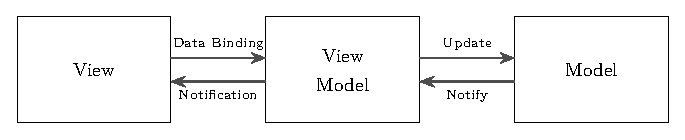
\includegraphics[width=0.78\textwidth]{figures/fig-mvvm.pdf}
  \caption{MVVM 原理图}
  \label{fig:mvvm}
\end{figure}

Model（模型）是指任何一个领域模型，代表一个面向对象的方法或者以数据为中心的数据访问层。它主要用于将应用程序中与业务逻辑相关的数据和该数据的处理方式进行封装，能够直接访问数据，例如对后台数据库的访问。Model 不依赖 View 和 View Model，即模型不关心被如何操作，也不包含任何用户界面的相关业务逻辑。

View（视图）是应用程序中用户可见的界面。视图对象不但了解如何将自己绘制出来，而且可能会对用户的操作做出相应的响应。视图对象的目的是显示来自应用程序模型对象的数据，并使该数据能够被编辑。尽管如此，通常情况下在 MVVM 应用程序中，视图对象与模型对象是分离的。

View Model（视图模型）是暴露公共属性与命令的视图的抽象，作为 View 与 Model 之间的桥梁，通过双向数据绑定把 View 层和 Model 层进行连接。开发者只需要关注业务逻辑的处理，因为 View 和 Model 之间的同步工作完全是自动的，无需人为干涉，无需手动操作 DOM 结点，也无需关注数据状态的同步问题。

（2）代理模式

代理模式（Proxy）主要用于为其他对象提供一种代理进而控制对这个对象的访问。代理模式使得代理对象能够控制具体对象的引用。代理几乎能够是任何对象：资源、文件、内存中的对象，或者是一些无法复制的东西。代理模式主要可以分为虚拟代理、缓存代理和用高阶函数动态创建代理三种。在 JavaScript 开发中最常用的是虚拟代理和缓存代理。

（3）观察者模式

观察者模式一般作为 Model 层对 View Model 的通知方式，不在意哪一层接收，只需要负责发布信息。它定义了一种一对多的关系，实现了多个观察者对象同时对某一个主体对象的监听，只要这个主体对象的状态发生任何变化就会通知所有的观察者对象，使得观察者们能够自动更新。

（4）单例模式

单例就是保证每次只有一个实例，实现方法一般是先判断实例是否存在，如果存在，则直接返回；如果不存在，则创建后再返回，从而确保只有一个实例对象。在 JavaScript 中，单例从全局命名空间内提供一个唯一的访问点来访问该对象，被作为一个命名空间提供者。

\subsection{JSON 技术的使用}

JSON（JavaScript Object Notation）是一种轻量级的数据交换格式。它是基于 ECMAScript 的一种完全独立的文本格式，采用完全独立于任何编程语言的文本格式进行数据的存储，主要用来传输由序列化的值或属性值组成的数据对象。同时，JSON 因其简洁和清晰的结构层次成为目前较为理想的数据交换语言。它的官方 MIME 类型是 \texttt{application/json}，文件扩展名是 \texttt{.json}。

JSON 主要由两种结构构建：第一种是"名称/值"对的集合，以左花括号开始、以右花括号结束，每一个"名称"后有一个冒号，多个"名称/值"对之间使用逗号作为分隔符；第二种是值的有序列表，一个数组以左中括号开始、以右中括号结束，多个值之间使用逗号作为分隔符。其中，值可以是被双引号包裹的数字、字符串、布尔值、空值、数组或者对象，这些结构都可以互相嵌套。

\subsection{PMP 刷题系统界面的实现}

小程序中的界面主要通过两部分实现。首先完成界面的布局，然后通过网络请求得到数据并将数据填充在相对应的界面。

\subsubsection{典型界面布局}

界面主要都是通过以下部分来实现的。通过在 \texttt{app.json} 或者 \texttt{page.json} 文件中对小程序进行全局配置，可以决定窗口表现形式、页面的文件路径、多 tab 的设置、网络请求超时时间的设置等。通过 \texttt{pages} 指定小程序由哪些页面组成，通过 \texttt{window} 设置导航条的背景颜色、导航栏的标题、状态栏、窗口的背景色等。在 \texttt{.wxml} 文件中使用微信小程序封装的指定组件开发页面结构，在 \texttt{.wxss} 文件中设置页面结构样式，在 \texttt{.js} 文件中实现界面逻辑以及生命周期函数的合理使用。其结构如图 \ref{fig:homepage} 所示。

\begin{figure}[htbp]
  \centering
  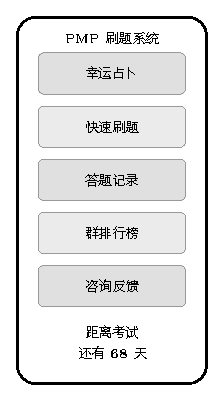
\includegraphics[width=0.30\textwidth]{figures/fig-homepage.pdf}
  \caption{刷题系统首页效果图}
  \label{fig:homepage}
\end{figure}

\subsubsection{数据填充}

首先，通过 GET 或者 POST 请求方式访问服务端的指定接口，获取相关的数据信息。其次，通过对服务端返回的数据进行 JSON 解析以及数据筛选，得到所需数据。最后，将不同接口的数据信息按照界面的布局渲染在相对应的组件上面，从而实现界面的数据填充。
